\documentclass{article}
\usepackage[T1]{fontenc}
\usepackage{lmodern}
\usepackage{graphicx}
\usepackage{amsmath,amssymb}
\usepackage[a4paper,margin=2cm]{geometry}
\usepackage[absolute,overlay]{textpos}
\setlength{\TPHorizModule}{1mm}
\setlength{\TPVertModule}{1mm}
\usepackage[indonesian]{babel}
\usepackage{hyperref}
\setlength{\emergencystretch}{2em}
% unit: Halaman 21

\begin{document}

% === Halaman 21 (llm) ===

Untuk citra dengan kontras rendah (seperti citra hasil fotografi), metode \textit{enhanced LSB} seringkali menyulitkan steganalisis. Karena steganalisis akan kesulitan membedakan antara gambar yang seharusnya muncul dengan pesan rahasia.\vspace{10mm}

\vspace{117.32mm}

Gambar III-3 Gambar dengan kontras rendah dan hasil \textit{enhanced LSB}-nya

% deskripsi: Perbandingan antara citra asli berupa bunga teratai (kontras rendah) di sisi kiri dan hasil pengolahan enhanced LSB yang terlihat seperti noise berwarna di sisi kanan.
% bbox normalisasi: [0.2020, 0.3720, 0.7520, 0.7670]
\begin{textblock*}{115.50mm}(42.42mm,110.48mm)
\noindent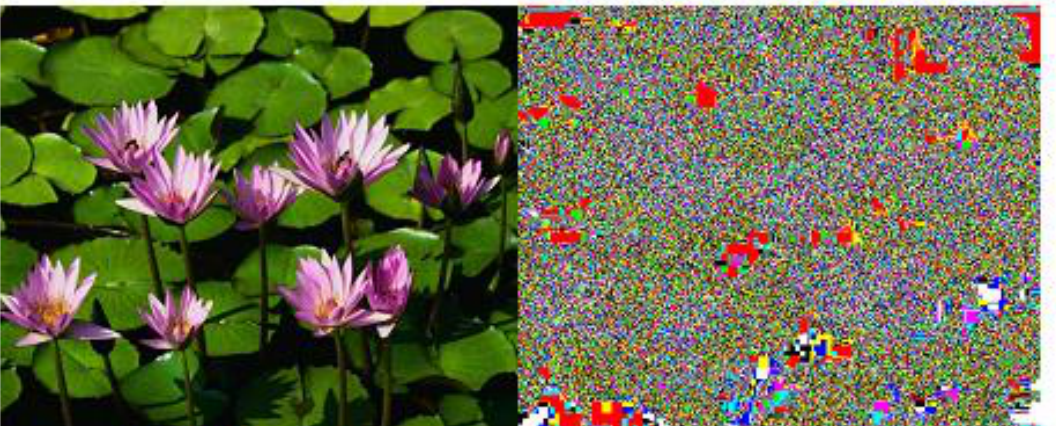
\includegraphics[width=115.50mm,height=117.32mm]{../../images/llm/page_021_img_01.png}%
\end{textblock*}

\end{document}
